\subsection{Design and Architecture}
\label{sec:design_arch}
% Design of your ITU-MiniTwit systems
% Architecture of your ITU-MiniTwit systems
% Important interactions of subsystems

The requirements of the \textit{Minitwit} system are well-defined. Hence, the design of the system is limited to the selection of the three-tier architecture.
\autoref{des-and-arch:fig:three-tier-arch} below depicts this architecture applied to the \textit{Minitwit} system.

\begin{figure}[H]
    \centering
    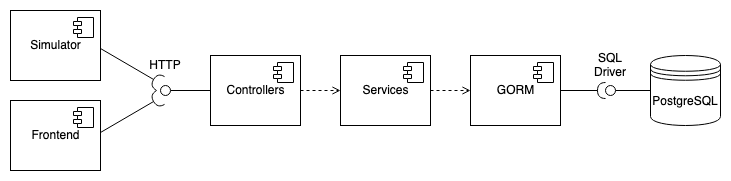
\includegraphics[width=\textwidth]{images/DevOpsArch.png}
    \caption{A high-level overview of \textit{Minitwit's} three-tier architecture}
    \label{des-and-arch:fig:three-tier-arch}
\end{figure}

Each layer is discretely bounded by communication interfaces.
The first layer consists of two clients to the \textit{Minitwit} system.
The frontend allows end-users to interact with the system, and the simulator replicates live users interacting with the system.
The second layer provides the core functionality of the \textit{Minitwit} system.
It exposes this functionality through two HTTP APIs, for the frontend and simulator respectively.
The third layer is a PostgreSQL database that provides the system with persistent data.

To implement the \textit{Services} component there is an important interaction with the \textit{GORM} component. \textit{GORM} is an object-relational mapper for Golang. The \textit{Services} component uses it as a bridge pattern to add a layer of abstraction such that several database vendors can provide persistence functionality.
\autoref{des-and-arch:fig:bridge-pattern} below reveals how the use of different SQL drivers allows \textit{Minitwit} to support different database vendors.

\begin{figure}[H]
    \centering
    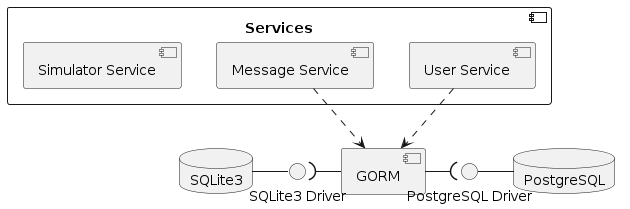
\includegraphics[scale=0.65]{images/DevOpsBridge.png}
    \caption{An illustration of \textit{Minitwit's} bridge pattern to support different database vendors}
    \label{des-and-arch:fig:bridge-pattern}
\end{figure}

